%%%%%%%%%%%%%%%%%%%%%%%%%%%%%%%%%%%%%%%%%%%%%%%%%%%
%% P3: Phenomenology of Particle Physics                         
%%
%% Author:  André Rubbia                   		 
%%
%% Figure 4.4 The Breit--Wigner probability density function $P(E)$ as a function of energy $E$.
%%
%% This work is licensed under the Creative Commons Attribution 4.0 International License. 
%% To view a copy of this license, visit http://creativecommons.org/licenses/by/4.0/ or 
%% send a letter to Creative Commons, PO Box 1866, Mountain View, CA 94042, USA.
%%
%%%%%%%%%%%%%%%%%%%%%%%%%%%%%%%%%%%%%%%%%%%%%%%%%%%

\documentclass[a4paper,10pt]{article}

\usepackage[T1]{fontenc}
\usepackage[utf8]{inputenc}
\usepackage{lmodern}
\usepackage[labelfont=bf]{caption}
\usepackage{upgreek}

\usepackage{tikz}
\usepackage{pgfplots}
\pgfplotsset{compat=1.17}
\usepgfplotslibrary{ternary}
\usepgfplotslibrary{fillbetween}
\usepgfplotslibrary{external}

\def\d{\mathrm{d}}

\begin{document}

%%%%%%%%%%%%%%%   FIGURE  %%%%%%%%%%%%%%%%%%%%%%%%%%%%%%
\begin{figure}[htb]
\begin{center}
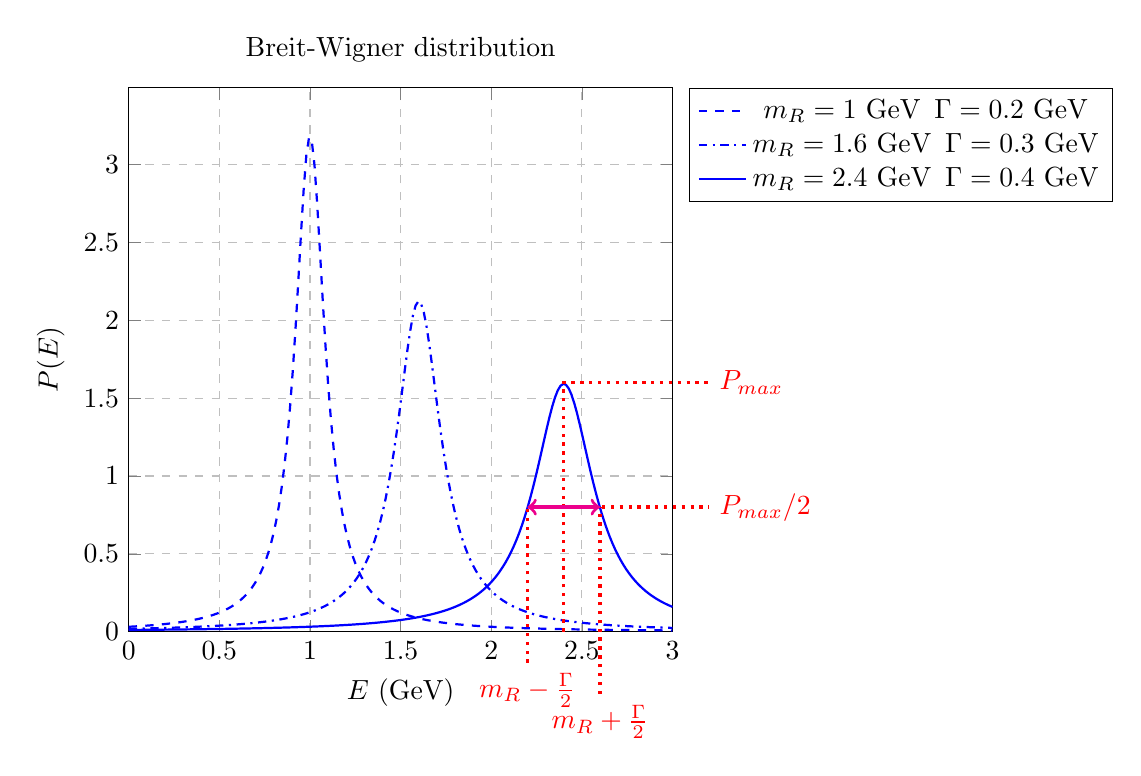
\begin{tikzpicture}[scale=1]
\begin{axis}[
   width=0.7\textwidth,
   height=0.7\textwidth,
    title={Breit-Wigner distribution},
    xlabel={$E$ (GeV)},
    ylabel={$P(E)$},
    xmin=0, xmax=3,
    ymin=0.0,
    %ymax=2,
%    xtick={0,20,40,60,80,100,120,140,160},
%    ytick={1e0,1e1,1e2,1e3,1e4,1e5,1e6,1e7},
    legend pos=outer north east,
    ymajorgrids=true,
    xmajorgrids=true,
    grid style=dashed,
    clip=false
]
\addplot[samples=200,domain=0:3,
    color=blue, thick, no marks,dashed
    ] { 0.2/(2*3.1415)/((x-1)^2+(0.2/2)^2)};
\addplot[samples=200,domain=0:3,
    color=blue, thick, no marks,dashdotted
    ] { 0.3/(2*3.1415)/((x-1.6)^2+(0.3/2)^2)};
\addplot[samples=200,domain=0:3,
    color=blue, thick, no marks
    ] { 0.4/(2*3.1415)/((x-2.4)^2+(0.4/2)^2)};
     \legend{$m_R = 1$~GeV\, $\Gamma=0.2$~GeV,
    $m_R = 1.6$~GeV\, $\Gamma=0.3$~GeV,
    $m_R = 2.4$~GeV\, $\Gamma=0.4$~GeV
    }
\draw[red, very thick, -, dotted] (axis cs:2.4,0) -- (axis cs:2.4,1.6) -- (axis cs:3.2,1.6) node[right] {$P_{max}$};
\draw[red, very thick, -, dotted] (axis cs:2.2,-0.2) node[below] {$m_R-\frac{\Gamma}{2}$} -- (axis cs:2.2,0.8) -- (axis cs:3.2,0.8) node[right] {$P_{max}/2$};
\draw[red, very thick, -, dotted] (axis cs:2.6,-0.4) node[below] {$m_R+\frac{\Gamma}{2}$} -- (axis cs:2.6,0.8) ;
\draw[magenta, very thick, <->] (axis cs:2.2,0.8)  -- (axis cs:2.6,0.8) ;
\end{axis}
\end{tikzpicture}
\caption{The Breit--Wigner probability density function $P(E)$ as a function of energy $E$. The value $\Gamma$
represents the full width at half maximum.}
\end{center}
\end{figure}
%%%%%%%%%%%%%%%   END FIGURE  %%%%%%%%%%%%%%%%%%%%%%%%%%%%%%
%

\end{document}
